\documentclass{oblivoir}
\usepackage{amsmath,amssymb,amsthm,kotex,mdframed,paralist,chngcntr}
\usepackage{kswrapfig}

\newcounter{num}
%\newcommand{\defi}[1]
%{\bigskip\noindent\refstepcounter{num}\textbf{정의 \arabic{num}) #1}\par}
%\newcommand{\theo}[1]
%{\bigskip\noindent\refstepcounter{num}\textbf{정리 \arabic{num}) #1}\par}
%\newcommand{\exam}[1]
%{\bigskip\noindent\refstepcounter{num}\textbf{예시 \arabic{num}) #1}\par}
\newcommand{\prob}[1]
{\bigskip\noindent\refstepcounter{num}\textbf{문제 \arabic{num}) #1}\par}
%\newcommand{\howo}[1]
%{\bigskip\noindent\refstepcounter{num}\textbf{숙제 \arabic{num}) #1}\par\bigskip}

\newcommand{\ans}{{\raggedleft\textbf{답 : (\qquad\qquad\qquad\qquad\qquad\qquad)}
\bigskip\bigskip\bigskip\par}}

\renewcommand{\proofname}{증명)}
\counterwithout{subsection}{section}


%%%
\begin{document}
\large

\title{승재 01 - 최고수준 수학}
\author{}
\date{\today}
\maketitle
%\tableofcontents
\newpage

%
\prob{p59, \#12-1}
어떤 물건을 원가의 0.4만큼 이익을 붙여 정가를 매겼습니다.
이 물건을 정가의 0.2을 할인하여 팔면 600원의 이익이 생긴다고 합니다.
이 물건의 원가는 얼마입니까?

5000원

\prob{p59, \#12-2}
어떤 물건을 원가의 0.25만큼 이익을 붙여 정가를 매겼습니다.
이 물건을 정가의 0.1을 할인하여 팔면 500원의 이익이 생긴다고 합니다.
이 물건의 원가는 얼마입니까?

4000원

\prob{p59, \#12-3}
철수는 어떤 물건을 사서 한 달 동안 사용한 뒤 친구인 영희에게 원래 가격의 절반의 가격으로 팔았습니다.
영희도 다시 한 달 동안 사용하다가 다시 철수에게 영희가 산 가격의 절반 가격으로 팔았습니다.
그동안 철수는 750원의 이익을 보았을 때 물건의 원래 가격은 얼마입니까?

1000원

%
\newpage

\prob{p62, \#07-1}
길이가 53m인 기차가 초속 32.5m로 달리고 있습니다.
이 기차가 길이가 450m인 터널을 완전히 통과하는 데 걸리는 시간은 약 몇 초인지 반올림하여 자연수로 나타내시오.

15초

\prob{p62, \#07-2}
`량'이란 전철이나 열차의 차량을 세는 단위입니다.
아래 그림처럼 생긴 열차의 경우 차량이 세 개 이어져 있으므로 3량입니다.

\begin{figure}[h]
\centering
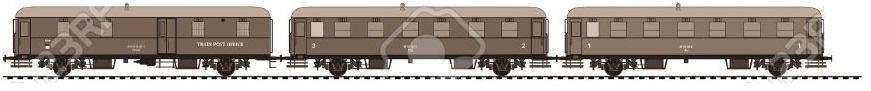
\includegraphics{6207-2}
\end{figure}

서울 지하철 5호선 지하철은 8량으로 되어 있고 한 량의 길이는 20m 입니다.
80 km/h로 달리는 5호선 열차가 길이 1240m의 천호대교를 완전히 건너는 데 걸리는 시간은 약 몇 초입니까?


63초

%
\newpage

\prob{p63, \#08-1}
\kswrapfig[Pos=r]{6308-1}{
떨어뜨린 높이의 0.8만큼 튀어 오르는 공이 있습니다.
오른쪽 그림과 같이 공을 떨어뜨렸을 때, 두 번째 튀어오른 높이는 바닥보다 65.6cm 높았습니다.
처음 공을 떨어뜨린 높이는 몇 cm입니까?

102.5cm
}


\prob{p63, \#08-2}
\kswrapfig[Pos=r]{6308-2}{
떨어뜨린 높이의 0.8만큼 튀어 오르는 공이 있습니다.
오른쪽 그림과 같이 공을 떨어뜨렸을 때, 두 번째 튀어오른 높이는 계단보다 36.4cm 높았습니다.
처음 공을 떨어뜨린 높이는 몇 cm입니까?

72.5cm
}

\prob{p63, \#08-3}
\kswrapfig[Pos=r]{6308-3}{
떨어뜨린 높이의 0.8만큼 튀어 오르는 공이 있습니다.
오른쪽 그림과 같이 공을 떨어뜨렸을 때, 두 번째 튀어오른 높이는 계단보다 66.08cm 높았습니다.
처음 공을 떨어뜨린 높이는 몇 cm입니까?

115cm
}

\end{document}